\usetikzlibrary{arrows.meta,shapes.geometric}%
\definecolor{mred}{RGB}{168,70,70}%
\definecolor{mgold}{RGB}{190,135,40}%
\definecolor{mblue}{RGB}{70,110,165}%
\definecolor{mgreen}{RGB}{80,140,90}%

\providecommand{\pbox}[1]{{\setlength{\fboxsep}{1.5pt}\setlength{\fboxrule}{0.25pt}\fcolorbox{black!25}{white}{\makebox[0.42cm][c]{\small\strut\textcolor{black!85}{#1}}}}}%

\providecommand{\panel}[5]{% #1 x-shift, #2 node prefix, #3 title, #4 folder (0/1), #5 member (0/1)
  \begin{scope}[shift={(#1,0)}]
    \draw[black!25, rounded corners=2pt, line width=0.4pt] (-1.3,-5.05) rectangle (1.3,0);
    \node[anchor=base, align=center, inner sep=0pt, font=\figurefont\small] at (0,0.2) {#3};
    \ifnum#4=1
      \ifnum#5=1 \def\fy{-3.175}\else\def\fy{-3.825}\fi
    \else
      \ifnum#5=1 \def\fy{-1.875}\else\def\fy{-2.525}\fi
    \fi
    \pgfmathsetmacro{\dy}{\fy+1.3}
    \pgfmathsetmacro{\ry}{\fy+2.6}
    \pgfmathsetmacro{\my}{\fy-1.3}
    \node[file] (#2f1) at (-0.75,\fy) {};
    \node[file] (#2f2) at (0.75,\fy) {};
    \draw[dep] (#2f1) -- (#2f2);
    \ifnum#4=1
      \node[folder] (#2root) at (0,\ry) {};
      \node[folder] (#2d1) at (-0.75,\dy) {};
      \node[folder] (#2d2) at (0.75,\dy) {};
      \draw[parent] (#2root) -- (#2d1);
      \draw[parent] (#2root) -- (#2d2);
      \draw[contains] (#2d1) -- (#2f1);
      \draw[contains] (#2d2) -- (#2f2);
    \fi
    \ifnum#5=1
      \node[member] (#2m1) at (-0.75,\my) {};
      \node[member] (#2m2) at (0.75,\my) {};
      \draw[dep] (#2m1) -- (#2m2);
      \draw[belongs] (#2m1) -- (#2f1);
      \draw[belongs] (#2m2) -- (#2f2);
    \fi
  \end{scope}
}%

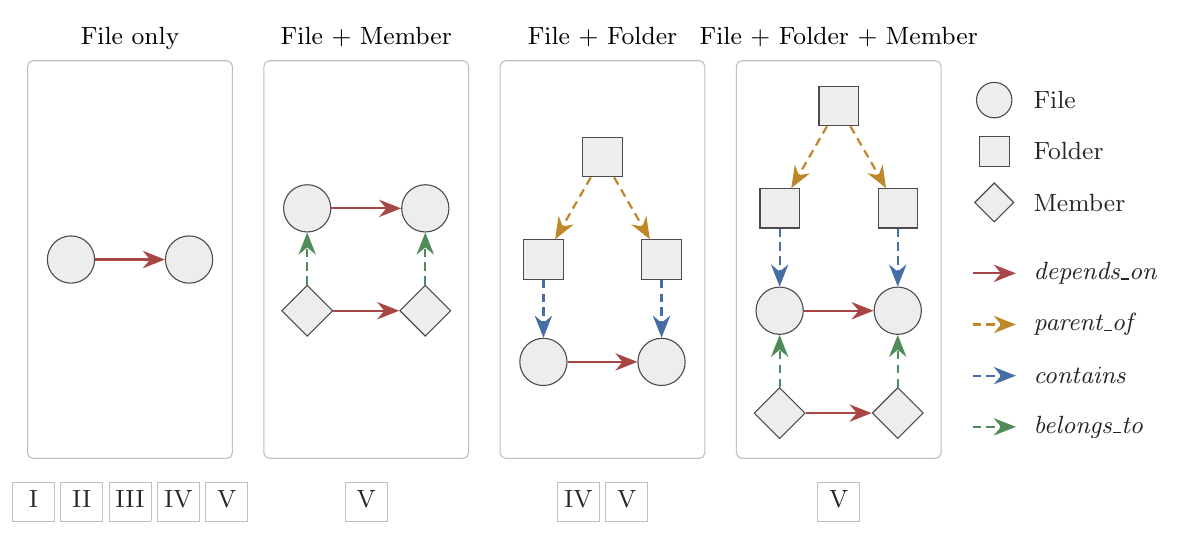
\begin{tikzpicture}[
  trim left=-1.3cm,
  font=\figurefont\normalsize,
  file/.style={circle, draw=black!70, fill=gray!14, minimum size=6mm, inner sep=0pt},
  folder/.style={rectangle, draw=black!70, fill=gray!14, minimum size=5mm, inner sep=0pt},
  member/.style={diamond, aspect=1, draw=black!70, fill=gray!14, minimum size=6.5mm, inner sep=0pt},
  lfile/.style={file, minimum size=4.5mm},
  lfolder/.style={folder, minimum size=3.8mm},
  lmember/.style={member, minimum size=5mm},
  dep/.style={-{Stealth[length=2.8mm,width=2.2mm]}, mred, thick},
  parent/.style={-{Stealth[length=2.8mm,width=2.2mm]}, mgold, thick, dash pattern=on 3pt off 2pt},
  contains/.style={-{Stealth[length=2.8mm,width=2.2mm]}, mblue, thick, dash pattern=on 3pt off 2pt},
  belongs/.style={-{Stealth[length=2.8mm,width=2.2mm]}, mgreen, thick, dash pattern=on 3pt off 2pt},
  legtext/.style={anchor=west, text=black!85, font=\figurefont\small}
]
  \panel{0}{a}{File only}{0}{0}
  \panel{3.0}{b}{File + Member}{0}{1}
  \panel{6.0}{c}{File + Folder}{1}{0}
  \panel{9.0}{d}{File + Folder + Member}{1}{1}

  % studies reporting results on each configuration (confirm FM, FF and FFM)
  \node at (0,-5.6) {\pbox{I}\hspace{2pt}\pbox{II}\hspace{2pt}\pbox{III}\hspace{2pt}\pbox{IV}\hspace{2pt}\pbox{V}};
  \node at (3.0,-5.6) {\pbox{V}};
  \node at (6.0,-5.6) {\pbox{IV}\hspace{2pt}\pbox{V}};
  \node at (9.0,-5.6) {\pbox{V}};

  % legend column: icons centered at x=10.975, text starts at x=11.35, last row at y=-4.65 (box bottom is -5.05)
  \node[lfile] at (10.975,-0.5) {};
  \node[legtext] at (11.35,-0.5) {File};
  \node[lfolder] at (10.975,-1.15) {};
  \node[legtext] at (11.35,-1.15) {Folder};
  \node[lmember] at (10.975,-1.8) {};
  \node[legtext] at (11.35,-1.8) {Member};

  \draw[dep] (10.7,-2.7) -- (11.25,-2.7);
  \node[legtext] at (11.35,-2.7) {\textit{depends\_on}};
  \draw[parent] (10.7,-3.35) -- (11.25,-3.35);
  \node[legtext] at (11.35,-3.35) {\textit{parent\_of}};
  \draw[contains] (10.7,-4.0) -- (11.25,-4.0);
  \node[legtext] at (11.35,-4.0) {\textit{contains}};
  \draw[belongs] (10.7,-4.65) -- (11.25,-4.65);
  \node[legtext] at (11.35,-4.65) {\textit{belongs\_to}};
\end{tikzpicture}%

